\documentclass[12pt]{article}
\usepackage[hidelinks]{hyperref}
\usepackage[a4paper]{geometry}
\usepackage[hang, labelfont=bf]{caption}
\usepackage{subcaption}
\usepackage{tikz}
\usepackage{float}
\usepackage{amsmath}
\usepackage{amssymb}
\usepackage{array}
\usepackage{qtree}
\usepackage[ruled, vlined]{algorithm2e}

\DeclareMathOperator*{\bigforall}{\mbox{\Large $\mathsurround0pt \forall$}}
\newcommand*{\p}{\ensuremath{\mathcal{P}}}
\newcommand*{\source}{\ensuremath{v_{src}}}
\newcommand*{\target}{\ensuremath{v_{target}}}
\newcommand*{\blocks}{\vdash}
\newcommand*{\blockedBy}{\dashv}
\newcommand*{\blockingScore}{B^+}
\newcommand*{\blockedScore}{B^-}


\setlength{\parindent}{0pt}
\setlength{\parskip}{1ex}

\author{
    \textsc{Jakub Pawlak}\\
    \href{mailto:j.pawlak@student.fontys.nl}{\texttt{j.pawlak@student.fontys.nl}}
    \and 
    \textsc{Grzegorz Malisz}\\
    \href{mailto:g.malisz@student.fontys.nl}{\texttt{g.malisz@student.fontys.nl}}
}

\title{\sffamily\bfseries\Huge Peking express optimal-strategy algorithm}

\begin{document}

\begin{titlepage}
    \newgeometry{left=1in, right=1in}
    \maketitle
    \thispagestyle{empty}
    \tableofcontents
    \restoregeometry
\end{titlepage}
\setcounter{page}{2}

\section{Introduction}

In the game 2 players take turns traversing a directed weighted graph.
One vertex is chosen as a destination and the aim of the game is to be the first player to reach that vertex.

Each player starts with the same budget --- every vertex has an associated travel cost, and each time a player traverses that edge, their budget decreases by that amount.
Players can only traverse an edge if their current budget is higher than the cost associated with that edge.

Additionally, some of the graph's vertices are \emph{critical locations}, meaning that they can only accomodate one player at a time.

An example map is shown on the fig.~\ref*{fig:example-map} below.
The start location is node $A$, marked in green, the target is node $D$ shown in red,
and the critical locations are marked with a double border, in this case only one being node $C$.

\begin{figure}[H]\centering
    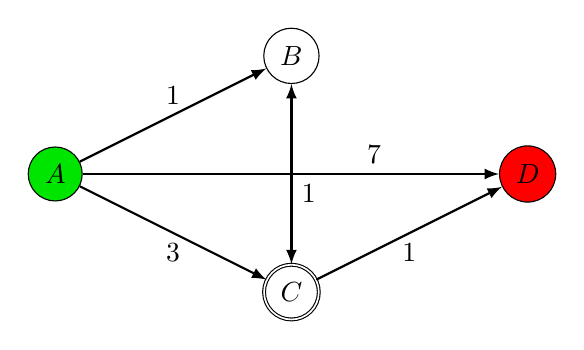
\begin{tikzpicture}[main/.style = {draw, circle}]
        \node[main, fill=green!90!black] (a) at (0,1.5) {$A$};
        \node[main, double] (c) at (3,0) {$C$};
        \node[main] (b) at (3,3) {$B$};
        \node[main, fill=red] (d) at (6,1.5) {$D$};

        \draw[-latex, thick] (a) -- (b) node[midway, above] {1};
        \draw[latex-latex, thick] (b) -- (c) node[midway, below right] {1};
        \draw[-latex, thick] (a) -- (c) node[midway, below] {3};
        \draw[-latex, thick] (a) -- (d) node[pos=0.7, above] {7};
        \draw[-latex, thick] (c) -- (d) node[midway, below] {1};
    \end{tikzpicture}
    \caption{Example map for the game with the source marked green and the target shown as red.}
    \label{fig:example-map}
\end{figure}

In each turn player can do one of the following:
\begin{enumerate}
    \item Travel to an adjacent vertex if the player's budget is higher than the cost of traversal
    \item Stay in the current location
\end{enumerate}

The assignment is to write an algorithm who will choose an optimal move given a game setting.

\section{Devising an algorithm}

\subsection{Resource constrained shortest path}

Consider a directed graph $G(V,E)$, where $V = \{v_1, \ldots , v_n\}$ represents a set of vertices,
and $E \subseteq \{ (i,j) \mid v_i \in V, v_j \in V, i \neq j \}$ a set of edges.
For each edge $(i,j) \in E$ there are 2 weights $c_{ij}$ and $t_{ij}$,
that represent the length and resource consumption of traversing the edge.

In the case of this game:
\begin{equation}
    \bigforall_{i,j} \; c_{ij} = 1
    \label{eq:all_cost_one}
\end{equation}
Because it takes just 1 turn to traverse an edge.

Consider a set $P$ of all simple paths possible in the graph $G$, and a set $P(\source,\target)$
of simple paths from $\source$ (source) to $\target$ (target).
For all $p \in P$ define the functions $C: P \to \mathbb{Z}^+$, and $R: P \to \mathbb{Z}^+$ as follows:
\begin{align}
    C(p) & = \sum\limits_{(i,j) \in p} c_{ij} \label{eq:len-func}  \\
    R(p) & = \sum\limits_{(i,j) \in p} t_{ij} \label{eq:cost-func}
\end{align}

The aim of the game is to reach the target in the shortest amount of moves while staying within the budget.
Therefore, we want to find such $p \in P(\source,\target)$ that minimizes the value of $C(p)$ while maintaing the condition $R(p) \leq t_{max}$.
This is the classic example of a well-known resource-constrained shortest path problem (RCSP).

\subsection{Critical location limitations}

\subsubsection{Blocking paths}

Now consider 2 simple paths: $p_a = (a_1, \ldots, a_n)$, and $p_b = (b_1, \ldots, b_k)$, where $a_n = b_k = \target$.
They will denote the shortest path chosen by each player respectively.

Since the critical loactions can only host one player at the time,
if both of the paths contain some critical location $c$, the players can block each other.

Assume player $a$ moves first.

In this case, path $p_a$ will block $p_b$, which we will denote as $p_a \blocks p_b$, if the following condition is met:
\begin{equation}
    p_a \blocks p_b \iff \exists i : a_i = b_i = c
\end{equation}
The opposite can occur, that is path $p_b$ will block $p_a$, denoted $p_a \blockedBy p_b$ if
\begin{equation}
    p_a \blockedBy p_b \iff \exists i : a_i = b_{i-1} = c
\end{equation}
This equation is an obvious consequence of the one above it, because after making a move, the path of the first player will ``shift'' to the left,
resulting in situation where the second player will be in a blocking advantage.

Additionally, if both conditions occur,
the one that occured first has a precedence,
that is, for some critical $c_1, c_2$:
\begin{equation}
    \exists i,j : (a_i = b_i = c_1 \land a_j = b_{j-1} = c_2) \implies
    \begin{cases}
        p_a \blocks p_b, \quad \text{if $i < j$}    \\
        p_a \blockedBy p_b, \quad \text{if $i > j$} \\
    \end{cases}
\end{equation}


\begin{figure}[H]\centering
    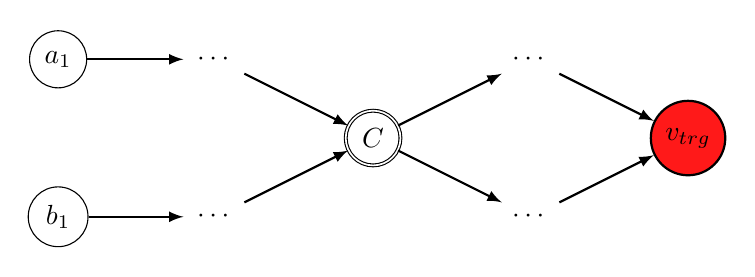
\begin{tikzpicture}[main/.style = {draw, circle}, ar/.style={thick, -latex}]
        % \node[main, fill=green!90!black] (start) at (0,0) {$S$};
        \node[main, double] (n) at (6,0) {$C$};
        \node[main, fill=red!90, thick] (target) at (10,0) {$v_{trg}$};


        \node[main] (a1) at (2, 1) {$a_1$};
        \node[circle] (a2) at (4, 1) {$\cdots$};
        \node[circle] (a3) at (8, 1) {$\cdots$};

        \node[main] (b1) at (2, -1) {$b_1$};
        \node[circle] (b2) at (4, -1) {$\cdots$};
        \node[circle] (b3) at (8, -1) {$\cdots$};

        % \draw[ar] (start) -- (a1);
        \draw[ar] (a1) -- (a2);
        \draw[ar] (a2) -- (n);
        \draw[ar] (n) -- (a3);
        \draw[ar] (a3) -- (target);

        % \draw[ar] (start) -- (b1);
        \draw[ar] (b1) -- (b2);
        \draw[ar] (b2) -- (n);
        \draw[ar] (n) -- (b3);
        \draw[ar] (b3) -- (target);
    \end{tikzpicture}
    \caption{Illurtration of two paths that might block}
\end{figure}


\subsection{Solving RCSP problem}

This problem can be solved in 2 approaches:
starting from source to all of the nodes reachable from it,
or starting from the target, to all of the nodes it is reachable from.

Since thrroughout the game the starting positions would stay the same,
but the target node $\target$ will be constant, we will use the second approach.

Let $z(a, t)$ be $\min \{ C(p) \mid p \in P(a,\target), T(p) \leq t \}$.
Then, we can define it to be

\begin{align}
    z(n,t) & = 0                                                   \\
    z(a,t) & = \infty \quad \text{if $a \neq \target$ and $t < 0$} \\
    z(a,t) & =
    \min\limits_{i : \exists (a,i) \in E}
    \Big\{
    z(i, t - t_{ai})
    \Big\}
\end{align}

This can be easily calculated using the dynamic programming approach, by filling in the table like the following:

\begin{table}\centering
    \begin{tabular}{|c|c c c c c c|}
        \hline
            & 0        & 1        & 2        & 3 & 4 & 5 \\ \hline
        $A$ & $\infty$ & $\infty$ & $\infty$ & 3 & 2 & 2 \\
        $B$ & $\infty$ & $\infty$ & 2        & 2 & 2 & 2 \\
        $C$ & $\infty$ & 1        & 1        & 1 & 1 & 1 \\
        $D$ & 0        & 0        & 0        & 0 & 0 & 0 \\ \hline
    \end{tabular}
    \caption{Example $z$ table for example from fig.~\ref{fig:example-map}}
\end{table}

Since each of the values of $z$ depends only on values for smaller $t$, we can fill this table going column-by-column.
The following algorithm accomplishes exactly that:

\begin{algorithm}[H]
    \DontPrintSemicolon
    \KwData{Directed graph $G(V,E)$,
        a set of weights $t_{ij}$ for each edge $i \to j$,
        target location $\target$,
        and starting budget $t_{max}$}
    \KwResult{A table $Z$ such that $Z[a][t] = z(a,t)$}
    \BlankLine
    \Begin {
        \For{$t = 0$ \KwTo $t_{max}$}{
            $Z[n][t] \longleftarrow 0$\;
            \ForEach{$a \in V, a \neq n$}{
                $z_{min} \longleftarrow \infty$\;
                \ForEach{$b \in V$, such that $(a,b) \in E$}{
                    \If{$t_{ab} \leq t$}{
                        $z_{new} \longleftarrow Z[b][t - t_{ab}] + 1$\;
                        $z_{min} = \min(z_{min}, z_{new})$
                    }
                }
                $Z[a][t] \longleftarrow z_{min}$\;
            }
        }
    }
    \caption{Algorithm to fill the table of $z_n(a,t)$}
\end{algorithm}

\subsection{Generating the shortest paths}

Let $\p(a,t)$ denote a set of all shortest paths from $a$ to $\target$, constrained by maximum resource usage $t$.
Since all of these paths are the shortest, all of them have the same length equal to $z(a,t)$.

Therefore, the set $\p(a,t)$ can be expressed as a follwing:

\begin{equation*}
    \p(a,t) = \big\{ p \in P(a,\target) \mid C(p) = z(a,t) \big\}
\end{equation*}

The above definition, however, does not give a way of efficient construction of such set.
It would require

Let us define a set $N_{viable}(a,t)$ of viable next moves from $a$ as a neighbourhood of vertex $a$, such that
every vertex in this set is closer to the target than $a$.
\begin{equation}
    N_{viable}(a,t) = \big\{ v \in N(a) , z(v,t-t_{av}) < z(a, t) \big\}
\end{equation}
where $N(a)$ is a neighbourhood of $a$, i.e.\ a set of all vertices adjacent to $a$.

The algorithm of selecting all that viable next moves is presented below:

\begin{algorithm}
    \DontPrintSemicolon
    \SetKwFunction{FViable}{Viable}
    \SetKw{KwYield}{yield}
    \SetKwProg{Fn}{Function}{:}{}
    \Fn{\FViable{a,t}}{
    \ForEach{$b \in N(a)$}{
    \If(\tcc*[f]{Can afford}){$t_{ab} \leq t$}{
    \If(\tcc*[f]{Closer to target}){$z(b, t-t_{ab}) < z(a,t)$}{
    \KwYield{$b$}\;
    }
    }
    }
    }
    \caption{Algorithm for generating all of the next viable moves}
    \label{alg:viable_next_moves}
\end{algorithm}

Now, we can define $\p(a,t)$ with a recursive formula.
The base case will be if we have reached the target, or if we do not have enough money to get to the target.
In other case, we will consider all of the viable vertices $v \in N(a,t)$, and for each of them every path we can take from there.
\begin{equation}
    \p(a,t) =
    \begin{cases}
        \big\{ (T) \big\}, \quad \text{if $a = T$}     \\[1ex]
        \;\emptyset, \quad \text{if $z(a,t) = \infty$} \\[1ex]
        \bigcup\limits_{v \in N_{viable}(a,t)} \Big\{ a::p \mid p \in \p(v, t-t_{av}) \Big\}
    \end{cases}
\end{equation}

Where $a :: p$ will denote path of taking $a$, followed by path $p$.
Formally:
\begin{equation*}
    a :: (p_1, p_2, \ldots, p_n) = (a, p_1, p_2, \ldots, p_n)
\end{equation*}

Below is the algorithm that will generate this set of paths:

\begin{algorithm}[H]
    \DontPrintSemicolon
    \SetKw{KwYield}{yield}
    \SetKwFunction{FPaths}{Paths}
    \SetKwFunction{FCombine}{Combine}
    \SetKwFunction{FViable}{Viable}
    \SetKwProg{Fn}{Function}{:}{}
    \KwData{Graph $G(V,E)$,
        a set of weights $t_{ij}$ for each edge $i \to j$,
        target location $\target$,
        starting position $a$
        and starting budget $t$}
    \KwResult{A set $\p(a,t)$ of shortest paths from $a$ to $\target$ not exceeding the budget $t$}
    \BlankLine
    \Fn{\FPaths{$a,t$}}{
        \uIf{$a = \target$}{
            \KwYield{$(\target)$} \tcc*{Reached the target}
        }
        \Else{
            \ForEach{$b \in \FViable{a,t}$}{
                $P \longleftarrow \FPaths{b,t}$\;
                \ForEach{$p \in P$}{
                    $p' \longleftarrow \FCombine{a,p}$\;
                    \KwYield{$p'$}\;
                }
            }
        }
    }
    \caption{Algorithm for generating all of the available shortest paths within a budget}
    \label{alg:shortest_paths}
\end{algorithm}

\subsection{Choosing the best path}

Having generated the set $\p(a,t)$, if there is more than one element in this set,
we are presented with a problem of which path to choose.

\subsubsection{Blocking analysis greedy approach}

For this method of choosing the best paths, we want to check how the paths player $a$ can take,
interact with the paths that player $b$ can take.

To accomplish this, we will examine the critical locations and see for which path combinations blocks occur.
Therefore, as our heuristic for choosing the best path we will use the probabilities of player $a$ blocking $b$ and vice versa.
Since the total number of shortest paths any player can choose is constant, instead of probabilities we will use just raw counts,
however keep in mind that the nature of this heuristic is still probabilistic.

Consider a situation of player $a$ being at vertex $v_a$ with budget $t_a$,
and player $b$ at vertex $v_b$ with budget $t_b$
For each path $p_a \in \p(v_a, t_a)$, we will define 2 metrics in the following way:
\begin{align}
    \blockingScore(p_a) & = \big| \{ p_b \in \p(v_b,t_b) \mid p_a \blocks p_b \} \big| \label{eq:blocking_score}   \\[.5ex]
    \blockedScore(p_a)  & = \big| \{ p_b \in \p(v_b,t_b) \mid p_a \blockedBy p_b \} \big| \label{eq:blocked_score}
\end{align}

It is obvious that the player $a$ would want to maximize the value of $\blockingScore$,
while minimizing the value of $\blockedScore$.
However, these values no not have a simple inverse relationship --- the increase of one does not necessarily mean the decrease of the other.
This poses the question --- which value we consider to be of greater importance.
There are two strategies one could take: a more aggressive one, where one tries to firstly maximize the $\blockingScore$ to try to block the other player,
or a more defensive one --- where one tries to minimize the $\blockedScore$ thus trying to avoid being blocked.

We have decided to be conservative in our approach, and assume that the other player will make the best move they can.
In this case, if the chances of the first player blocking them are not certain, they will probably choose an alternative path.
For this reason, unless probability of player $a$ blocking $b$ is not certain, the aggressive strategy is not the best option.

Therefore, we decided to firstly choose the path with minimal $\blockedScore$,
and if we still have a choice left, only then tries to maximize the $\blockingScore$.
Note that if there exist a path that will with $100\%$ certainty block player $b$,
which as we established was the only time it is viable to play aggressively, our approach will choose that option.

Note that this algorithm is not guaranteed to reult in the totally best result, 
however, supported by the fact that the paths we choose from are already the shortest paths possible,
and the applied heuristics are only aimed to even further improve the choice, we are satisfied with the result.

As of calculating the scores $\blockingScore$, and $\blockedScore$, the only difficult part is determining how paths block each other.
The algorithm for this is presented below:

\begin{algorithm}[H]
    \DontPrintSemicolon
    \SetKwFunction{Flen}{len}
    \KwData{Pats $p_a$ and $p_b$, with $p_a$ being the path of the player who is first to move, and a set $C$ of critical locations}
    \KwResult{Blocking relationship between $p_a$ and $p_b$: either $p_a \blocks p_b$, or $p_a \blockedBy p_b$, or no block}
    \Begin{
    \For{$i = 0$ \KwTo $\Flen(p_a)$}{
    \uIf{$p_a[i] = p_b[i]$}{
    \KwRet{$p_a \blocks p_b$}\;
    }\ElseIf{$p_a[i] = p_b[i-1]$}{
    \KwRet{$p_a \blockedBy p_b$}\;
    }
    }
    \KwRet{no block}\;
    }
    \caption{Algorithm for checking the blocking relations between two paths}
    \label{alg:paths_blocking}
\end{algorithm}

Having this, determining the scores $\blockingScore$ and $\blockedScore$ is trivial.

\subsubsection{Minimax}

The game has 3 possible outcomes:
\begin{enumerate}
    \item $a$ wins
    \item tie
    \item $b$ wins
\end{enumerate}
They are listed in that order for a reason.
From a perspective of player $a$, he would prefer the first outcome over second, and the second over third.
The player $b$ on the contrary, he would prefer outcome 3 over 2, and 2 over 1.

We can see that we can clearly form a poset of this outcomes.
Let's change the numbers a bit and say that the result is $+1$ if $a$ wins, $-1$ if $b$ wins, and 0 in case of a tie.
It is now clear that if a player is presented with a set of outcomes, 
player $a$ will try to maximize the outcome, 
while player $b$ will try to minimize it.

This enables us to recursively evaluate any of the available moves.
The best move player $a$ can make is the one that maximizes the minimum score of all the moves player $b$ can make after.

This is a well known problem in game theory, very common in turn-based games.

To better visualize the problem, it might be helpful to imagine the possible moves as a tree, like in fig.~\ref{fig:minimax-visualisation}.
Each of the tree levels represents a player turn, where one player will try to choose the minimum value of its children, while the other one will choose the maximum.
Therefore, knowing only the end scores, as in fig.~\ref{fig:minimax-empty}, we can calculate the best score one can reach from any position, 
by taking minimum and maximum alternately.
The result of this is shown on fig.~\ref{fig:minimax-full}.

\vspace*{1em}

\begin{figure}[H]\centering
    \begin{subfigure}[ht]{0.4\textwidth}
        \Tree [
            .$\max$ 
            [.$\min$ [.$\max$ -2 5 ] [.$\max$ 1 -3 ] ]
            [.$\min$ [.$\max$  4 1 ] [.$\max$  2 0 ] ] 
        ]
        \caption{}
        \label{fig:minimax-empty}
    \end{subfigure}
    \begin{subfigure}[ht]{0.4\textwidth}
        \Tree [
            .2 
            [.1 [.5 -2 5 ] [.1 1 -3 ] ]
            [.2 [.4  4 1 ] [.2  2 0 ] ] 
        ]
        \caption{}
        \label{fig:minimax-full}
    \end{subfigure}
    \caption{Illustration of the outcomes each player will choose}
    \label{fig:minimax-visualisation}
\end{figure}

In our case this tree can grow very big, therefore,
for performance considerations, we might want to limit the maximum depth.
This depth will be the number of moves the algorithm examines.
For example for depth 5, the algorithm will examine every possible position at 5 moves ahead.

For the purpose of limiting the depth, 
we need to estimate a heuristic for a situation where we reach maximum tree depth 
but game has not ended yet.
A sufficiently good estimate can be made with the table of $z$ values we have calculated.
We just check the shortest distance of each player to the target vertex and calculate their difference.

Therefore, our heuristic will be:
\begin{equation}
    h(v_a, t_a, v_b, t_b) = z(v_b, t_b) - z(v_a, t_a)
\end{equation}
Therefore if $h > 0$, the player $a$ is closer to the target than $b$.
If $h > 0$, player $b$ is closer, and if $h = 0$, they are equally close.

By introducing this heuristic we will again need to modify the evaluation values of end game states ---
player $a$ will obviously prefer to win, than be 2 edges closer than $b$.
Therefore, we will leave the tie at 0, 
but situation when $a$ wins we will assign $+\infty$, 
and when $b$ wins, $-\infty$.

Thanks to this, we can statically evaluate every position, and therefore, 
we can use a popular minimax algorithm, which looks the following:

\begin{algorithm}[H]
    \DontPrintSemicolon
    \SetKwFunction{Fminimax}{minimax}
    \SetKwFunction{Fmin}{min}
    \SetKwFunction{Fmax}{max}
    \SetKwData{false}{FALSE}
    \SetKwData{true}{TRUE}
    \SetDataSty{ttfamily}
    \SetKwProg{Fn}{function}{:}{}
    \Fn{\Fminimax{position, depth, maximizingPlayer}}{
        \If{$depth = 0$ or game over in position} {
            \KwRet{static evaluation of position}
        }
        \uIf{maximizingPlayer}{
            $maxEval \longleftarrow -\infty$\;
            \ForEach{next position}{
                $eval \longleftarrow$ \Fminimax{next, $depth - 1$,\false}\; 
                $maxEval \longleftarrow$ \Fmax{eval, maxEval}\;
            }
            \KwRet{$maxEval$}\;
        }\Else(\tcc*[f]{minimizing player}){
            $minEval \longleftarrow \infty$\;
            \ForEach{next position}{
                $eval \longleftarrow$ \Fminimax{next, $depth - 1$,\true}\; 
                $minEval \longleftarrow$ \Fmin{eval, maxEval}\;
            }
            \KwRet{$minEval$}\;
        }
    }
    \caption{General scheme of minimax algorithm}
    \label{alg:minimax_basic}
\end{algorithm}

\end{document}